% !TEX program = xelatex
\documentclass[10.5pt,a4paper,headings]{ctexart}
\usepackage{titling}
\usepackage{metalogo}

% \author{16-1-whoami?}
%
%Margin - 1 inch on all sides
%
\usepackage[letterpaper]{geometry}
\usepackage[OT2,T1]{fontenc}
\usepackage{inconsolata}
\usepackage{subfigure}
\usepackage{float}
\usepackage{pdfpages}
\usepackage{csquotes}
\usepackage{svg}
\usepackage{minted}
\usepackage{bm}
\usepackage{xltxtra,xunicode}
\geometry{a4paper,top=1.0in, bottom=1.0in, left=1.0in, right=1.0in}


% array for tabular width
\usepackage{array}

% xeCJK package to resolve CJK font family by yourself.
% \usepackage{xeCJK}
% \setCJKmainfont[BoldFont=SourceHanSerifSC-SemiBold, ItalicFont=STKaiti]{SourceHanSerifSC-Regular}
% \setCJKsansfont[BoldFont=SourceHanSansSC-Bold]{SourceHanSansSC-Regular}
% \setCJKmonofont{NotoSansMonoCJKsc-Regular}

% %

\ctexset{
section/format=\textbf{}\zihao{-4}\raggedright,
subsection/format=\zihao{-4}\raggedright,
}

% times new roman for ascii
\usepackage{times}

%Doublespacing
\usepackage{setspace}
\doublespacing
%\onehalfspacing

\usepackage{enumerate}

%Rotating tables (e.g. sideways when too long)
\usepackage{rotating}
\usepackage{fancyhdr}
\usepackage{indentfirst}
\usepackage{graphicx}
\usepackage{etoolbox}
\AtBeginEnvironment{minted}{\onehalfspacing
\fontsize{10.5}{13}\selectfont}

%
%Fancy-header package to modify header/page numbering (insert last name)
%
\pagestyle{fancy}
\lhead{}
\chead{}
\rhead{\XeLaTeX \ \ \thepage}
\lfoot{}
\cfoot{}
\rfoot{}
\renewcommand{\headrulewidth}{0pt}
\renewcommand{\footrulewidth}{0pt}

%To  sure we actually have header 0.5in away from top edge
%12pt is one-sixth of an inch. Subtract this from 0.5in to get headsep value
\setlength\headsep{0.333in}
\newcommand{\titleline}[1]{\hspace*{6em} #1 \\}
\newcommand*{\blankpage}{%
\vspace*{\fill}
{\centering\fontsize{32pt}{64pt} This page is intentionally left blank.\par}
\vspace{\fill}}
\makeatletter
\renewcommand*{\cleardoublepage}{\clearpage\if@twoside \ifodd\c@page\else
\blankpage
\thispagestyle{empty}
\newpage
\if@twocolumn\hbox{}\newpage\fi\fi\fi}

%
%Works cited environment
%(to start, use \begin{workscited...}, each entry preceded by \bibent)
% - from Ryan Alcock's MLA style file
%
\newcommand{\bibent}{\noindent \hangindent 40pt}
\newenvironment{workscited}{\newpage \begin{center}参考文献
\end{center}}{\newpage }

% \newcommand{\fs}{\CJKfamily{fs}}

%
%Begin document
%
\begin{document}
\begin{titlepage}
\scshape


% Cover page
\begin{center}
\vspace*{0.6cm}

\includegraphics[width=0.65\textwidth]{./logo.jpg}

\doublespacing
\fontsize{18pt}{2em}\bf
本科学生实验(实践)报告\\
\vspace{1em}
院系:计算机学院
\hspace{2ex}
软件学院
\end{center}

\begin{flushleft}

\setlength{\parindent}{2em}
\bf
{\fontsize{14pt}{18pt}
% \doublespacing

\linespread{1.5}\selectfont
~\\
\titleline{实验课程:科技文献阅读与写作}

\titleline{实验项目:符合华南师大一般要求的实验报告封面}

\titleline{指导老师:PhD. Zhu}
~\\
\titleline{开课时间:2018 ~ 2019年度第 1 学期}

\titleline{专\hspace{2em}业:网络工程}

\titleline{班\hspace{2em}级:16级 1 班}

\titleline{姓\hspace{2em}名: 王老五}

\titleline{学\hspace{2em}号:20112101010}
}
\end{flushleft}

% Footer
\begin{center}
\vspace{3cm}
\fontsize{14pt}{21pt}
\bf 华南师范大学教务处
\end{center}

\end{titlepage}

\blankpage
\newpage
% table
\tableofcontents

\newpage

%%%%Title
\begin{center}
\zihao{3}
\tt 符合华南师大一般要求的实验报告封面
\end{center}

%%%%Changes paragraph indentation to 2em (2 CJK character)
\setlength{\parindent}{2em}

%%%%Begin body of paper here

%% abstract
\onehalfspacing
【摘要】本实验报告封面是一般性的实验报告封面,符合一般的实验要求,例如计算机学院本科的诸多实验报告。本模板尚未结构化,仅作为一般模板使用。如产生学术纠纷与损失,本模板及其贡献者概不负责。

\doublespacing
\section{概述}
本实验报告模板处于一般状态,尚未很好地进行结构化整改。课业繁忙,难以寻找时间进行整改。作为单文件模板使用,是没有问题的。

\section{编译环境}
本模板的编译环境为\XeLaTeX ,使用了ctex作为基础类,这是由于\XeLaTeX 对Unicode有直接的支持,以实现编译中文。诸多的命令可以参考ctex文档。

\section{自定义字体}
文档可以使用\texttt{xeCJK}宏包来自定义字体,以使用自己的字体例如微软雅黑等。

\section{目录}
解除注释 \texttt{table of content} 行可以实现自动添加目录,在生成目录的时候需要使用\XeLaTeX 编译两遍。

\section{代码}
如果需要使用代码功能,需要将\texttt{$\backslash$usepackage\{minted\}}行解除注释并在其中添加:
\begin{minted}[mathescape,
linenos,
numbersep=6pt,
frame=lines,
framesep=2mm]{json}
"--shell-escape"
\end{minted}

\section{图片}
图片的使用是非常一般的,但需留意自动生成的图片顺序。
\begin{figure}[htbp]
\centering
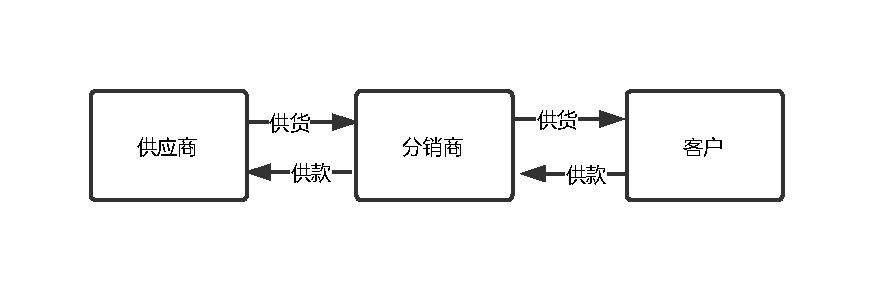
\includegraphics[page=1,width=0.75\textwidth]{f1.pdf}
\caption{图片示例}
\end{figure}

\section{表格}
利用array宏包,自定义表格宽度。横线用hline给出,竖线在tabular上用竖线给出。同时必须留意表格的每一行都要用两个反斜杠$\backslash\backslash$隔开。

\begin{table}
\centering
\begin{tabular}{ | p{1.5cm}<{\centering} | p{2cm}<{\centering} | p{3cm}<{\centering} | p{5cm}<{\centering} |}
\hline
key         & type      & description       & constraint \\
\hline
sid         & INT       & id of salesman    & PRIMARY KEY AUTO\_INCREMENT  \\
\hline
s\_name      & VARCHAR   & name of salesman  & UNIQUE  \\
\hline
s\_email     & VARCHAR   & email             & UNIQUE \\
\hline
password    & VARCHAR   & SHA3-256          & \\
\hline
\end{tabular}
\caption{TABLE salesman}
\end{table}

\begin{workscited}

\bibent
参考文件引用了MLA style模板,如果不喜欢,可以注释掉并且使用\texttt{thebibliography}宏包。

\bibent
Baker, Gladys L., Wayne D. Rasmussen, Vivian Wiser, and Jane M. Porter. \textit{Century of Service: The First 100 Years of the United States Department of Agriculture.}[Federal Government], 1996. Print.

\bibent
Danhof, Clarence H. \textit{Change in Agriculture: The Northern United States, 1820-1870.} Cambridge: Harvard UP, 1969. Print.

\bibent
张三,李四:椰子的一百种吃法,《中国椰子协会》第一期02~12页

\end{workscited}

\end{document}
